\quad Nakon što smo selekcijom dobili roditelje budućih programa, operacijom križanja pokušavamo stvoriti djecu ispreplećući roditeljske gene. U CGP-u ne radimo sa stablima već s mrežama što nas potiče na drukčiji pristup od onog opisanog u 3. poglavlju. U ovom poglavlju opisuje se križanje u CGP-u, utjecaj operacije na uspješnost programa i neki od načina implementacije.

\par
Križanje u CGP-u jako je zanimljiva tema. Tema koja se još uvijek istražuje i koja dobar dio vremena nije bila u fokusu. Primjenom operacije u nekim slučajevima dobivamo bolje rezultate nego kad se operacija ne primjenjuje, ali u nekim slučajevima i gore. Način implementacije znatno utječe na djelotvornost operacije \cite{CGPbook}\cite{CGPpresentation}. Zato se križanju, posebice u CGP-u, pristupa jako pažljivo i nerijetko se izbjegava. Križanje može biti snažan alat koji će spojiti najbolje dijelove roditelja ili alat koji će poremetiti ono što je roditelje činilo uspješnim.
\par
Originalni pokušaj ostvarenja križanja u CGP-u donekle je jednostavan. U mreži možemo odabrati nasumični gen te na mjestu odabranog gena presjeći obje kopije roditelja. Potom uzimamo prvi dio prve kopije i spajamo ga s drugim dijelom druge kopije, a zatim spajamo drugi dio prve kopije s prvim dijelom druge kopije. Vizualizaciju ovog procesa možemo vidjeti na slikama 6.1(a)-6.3(b).
\begin{figure}[h]
	\centering
	\begin{subfigure}{0.4\textwidth}
		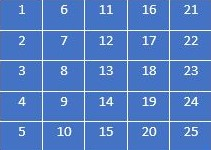
\includegraphics[width=0.9\linewidth]{cross_1} 
		\caption{Kopija prvog roditelja}
	\end{subfigure}
	\begin{subfigure}{0.4\textwidth}
		{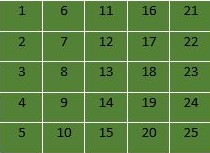
\includegraphics[width=0.9\linewidth]{cross_2}}
		\caption{Kopija drugog roditelja}
	\end{subfigure}
	\caption{Početne mreže roditelja }
\end{figure}

 \begin{figure}[h]
	\centering
	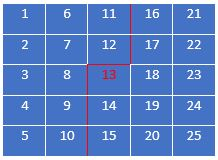
\includegraphics[width=0.4\linewidth]{cross_3}
	\caption{Odabir gena za presjek}
\end{figure}

\begin{figure}[h]
	\centering
	\begin{subfigure}{0.4\textwidth}
		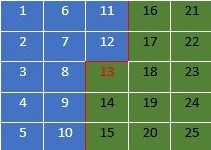
\includegraphics[width=0.9\linewidth]{cross_4} 
		\caption{Prvo dijete}
	\end{subfigure}
	\begin{subfigure}[b]{0.4\textwidth}
		{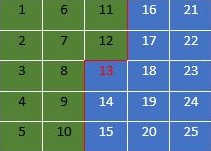
\includegraphics[width=0.9\linewidth]{cross_5}}
		\caption{Drugo dijete}
	\end{subfigure}
	\caption{Djeca nastala spajanjem dva dijela roditelja}
\end{figure}
\newpage
\par
Ovakav oblik križanja pokazao se izrazito destruktivnim u drugim radovima \cite{CGPbook}. Ipak, ovakav oblik križanja korišten je u ovom radu na mrežama širine jedan. Učinak takvog križanja na žalost nije provjeren u radu, križanje je provedeno u svim testovima. Ostavlja se kao potencijalna tema daljnjeg istraživanja. 
\par
Tijekom godina razvijeno je nekoliko drugih metoda među kojima se ističe metoda zamjene podgrafova aktivnih čvorova \cite{newcross}. Metoda je slična gore navedenoj metodi, ali ne dijelimo i ne spajamo sve gene grafa već samo one kodirajuće/aktivne što bi trebalo smanjiti destruktivnost i poremećaje u novim mrežama. 